\documentclass[letterpaper, 10 pt]{article}
\usepackage[spanish]{babel}
\usepackage[margin = 0.5 in]{geometry}
\usepackage[utf8]{inputenc}
\usepackage{multicol}
\usepackage{graphicx}
\usepackage{amsmath}
\usepackage{float}
\usepackage{caption}
\usepackage{hyperref}
\usepackage{natbib}

\hypersetup{
	colorlinks=true,
	linkcolor=black,
	urlcolor=black,
	filecolor=black,
	citecolor=blue,
	pdftitle= anotaciones clase
}


\newcommand{\fjsp}{problema de programación de taller de trabajo flexible}
\newcommand{\Tittle}[1]{ {\LARGE  #1 }  }
\newcommand{\subTittle}[1]{ {\Large  #1 }  }
\newcommand{\normalTittle}[1]{ {\normalsize  #1 }  }

\providecommand{\keywords}[1]
{
	\small	
	\textbf{\textit{Keywords---}} #1
}

\newenvironment{Figura}
{\par\medskip\noindent\minipage{\linewidth}}
{\endminipage\par\medskip}

\usepackage{enumerate}

\begin{document}

%\ttfamily %mecanografiada
%\rmfamily %Roman
\sffamily %sans

\begin{titlepage}
	\begin{center}
		\vspace*{1cm}
		
		\Tittle{UNIVERSIDAD AUTÓNOMA DE NUEVO LEÓN} \\
			\vspace{1.5 cm}
		\Tittle{FACULTAD DE INGENIERÍA MECÁNICA Y ELÉCTRICA} \\ 
		\vspace{1cm}
		{\LARGE Uso de Q-learning como alternativa a la solución del problema de programación de taller de trabajo flexible}
		\\
			\vspace{2.5 cm}
		
\includegraphics[width=0.3\textwidth]{uanl}
		 \\
		\vspace{1cm}
		\subTittle{Arnoldo Del Toro Peña}  \vspace{0.25 cm} \\ 
		\subTittle{Director de tesis:} \vspace{0.25 cm} \\
		\subTittle{Dr. Vincent Andre Lionel Boyer} 
		
		
		
		\vfill
		
		{\LARGE  Propuesta de Investigación\\
		Maestría en Ciencias de la Ingeniería con Orientación en Sistemas}
		
		\vspace{0.8cm}
		
		
		
		Monterrey, Nuevo León \\
		\today
		
	\end{center}
\end{titlepage}

\pagestyle{empty}
\tableofcontents

%\newpage
%\pagestyle{fancy}
%
%\newpage
%\thispagestyle{plain}
%
%\begin{center}
%	\large{\textbf{AGRADECIMIENTOS}}
%\end{center}
%
%Al Consejo Nacional de Ciencia y Tecnología (CONACYT) por el apoyo
%económico brindado durante la realización de mis estudios.
%
%Al Consejo, por haberme brindado la oportunidad de seguir
%mi formación académica en sus aulas.
%
%A los integrantes de mi Consejo Particular:
%
%Al Dr. Vincent mi más sincero agradecimiento, por sus
%atinadas indicaciones y consejos mismos que me fueron de gran utilidad en la
%realización del presente trabajo de tesis.
%
%A mis profesores, compañeros de clase y todas aquellas personas que de
%alguna manera me apoyaron en esta tarea, a todos gracias.

\newpage 
\begin{abstract}
	En esta propuesta de tesis, se propone el uso de una búsqueda de aprendizaje por refuerzo (Q-learning) en un problema de programación de taller de trabajo flexible. Se obtienen instancias a partir de la literatura, el planteamiento metodológico de una búsqueda de soluciones basándose en el algoritmo aprendizaje por refuerzo (Q-learning), resultados con base en un algoritmo genético (Genetic Algorithm) y la discusión de los posibles resultados de una búsqueda de aprendizaje por refuerzo (Q-learning). 
	
	In this thesis proposal, the use of a reinforcement learning search (Q-learning) in a flexible job shop scheduling programming problem is proposed. Instances were obtained from the literature, the methodological approach of a search for extreme solutions in the reinforcement learning algorithm (Q-learning), results based on a genetic algorithm and the discussion of the possible results of a quest for reinforcement learning (Q-learning).
		
	% It's  a brief summary of approximately 300 words. It includes the important questions, the rationale for the study, the hypothesis, the method, and the other characteristics. When describing the method, the design, procedure, results, and discussion must be included.
\end{abstract}

{{\small } \bfseries Palabras clave---} Aprendizaje por refuerzo, metaheurístico, python \\
\keywords{Q-learning, metaheuristic, python}

%\section{Justificación}
%En los últimos años se ha visto el crecimiento de la inteligencia artificial en diferentes áreas de la ciencia y en particular en el área de investigación de operaciones.
%% In this section, the research proposal must be justified.
%
%\section{Objetivo}
%Evidenciar si es viable un método basado en búsqueda Q-learning como alternativa a un método metaheurístico para la solución a un \fjsp.
%% Describe clearly and concisely the objective of your research proposal.

\section{Introducción}
% motivación
En los últimos años se puede decir que ha existido un uso casi exclusivo de métodos exactos y metaheurísticos en el área de investigación de operaciones, dejando de lado el campo que a tomado mucho auge estos últimos años a favor de la inteligencia artificial, es por eso que existe el motivo de una implementación de inteligencia artificial en esta misma área.

% Oportunidad
Esto representa una oportunidad interesante al momento de pensar en alternativas a métodos metaheurísticos, lo cual contiene la circunstancia de implementar un aprendizaje por refuerzo (Q-learning), 
%Innovación
siguiendo esta posibilidad se busca la actualización a las emergentes tecnologías como lo es la inteligencia artificial con el fin de lograr la innovación en métodos de aproximación en el campo de la investigación de operaciones.

%Pregunta y problema
La pregunta principal que se aborda es la siguiente: ¿Es viable utilizar la búsqueda aprendizaje por refuerzo (Q-learning) en el \fjsp?, y de ser así ¿Bajo que condiciones es favorable utilizar una búsqueda aprendizaje por refuerzo (Q-learning)?, bajo estas cuestiones se plantea la hipótesis: ``El aprendizaje por refuerzo (Q-learning) es una alternativa de calidad satisfactoria para obtener una solución al \fjsp", esto define como propósito principal generar evidencia fundamentada para descartar o aceptar la hipótesis antes definida, y con objetivo específico en el problema de programación de taller de trabajo flexible. 

% Estructura No se debe de dejar duda de que se va hacer y como se va a hacer
En las secciones siguientes se encuentran: la descripción de la literatura consultada, el marco metodológico, resultados, conclusiones y las respectivas referencias bibliográficas. En la sección de la literatura se tiene un pequeño resumen de los artículos más relevantes para nuestro estudio, en el marco metodológico se describe el proceso y procedimientos llevados a cabo, llegando al apartado de resultados se presentan los datos obtenidos hasta este momento y por último se finaliza con una sección para presentar conclusiones.


\section{Marco teórico}
% definir todos los conceptos utilizados, en que punto se encuentra la ciencia en nuestro experimento, información pertinente, seleccionada, ordenada y jerarquizada de manera que el lector pueda ubicar la investigación en su contexto teórico
%Antecedentes y contexto.
%Revisión de literatura.
%Tomando en cuenta la actual literatura que tenemos; existen muchos artículos que hablan de ``Q-learning'' aplicadas a la solución de problemas de ruteo, asignación, entre otras; sin embargo hasta el día de hoy no se ha encontrado ningún documento que presente un análisis en contraste con el uso de métodos metaheurísticos, por lo cual nos motiva a seguir pero también a tener precaución, ya que queda una pregunta en el aire, ¿Será útil la comparación?
%
%Lo que se quiere expresar es que el hecho de no haber tantos artículos puede ser debido a los carentes resultados comparados con los correspondientes de métodos metaheurísticos, por el excesivo tiempo de aprendizaje o tal vez por algún otro factor negativo hacia el aprendizaje ``Q-learning''.

%#FIXME cambiar antecedentes a estado del arte, y en antecedentes agregar libros que tengan que ver con métodos o procesos de tu tesis
%En los resultados presentados por Chen \textit{et al.} \cite{CHEN2022939}, se presentan los detalles de la implementación Deep Q-Learning, los resultados analíticos junto con pruebas, ilustraciones de la toma de decisiones, combinaciones de funciones adicionales, un análisis del valor de no ofrecer el servicio y los resultados para expandir las decisiones de asignación. Además se utilizó una estructura básica para cada una de las tres etapas: Input Layer, Hidden Layer and Output Layer. El artículo presenta variables de drones, vehículos terrestres y no prestar el servicio, cada una de estas variables es analizada a lo largo del artículo. Se presentan unos resultados muy favorables a las ecuaciones planteadas (Q-learning), pero no compara sus resultados con algún método metaheurístico, en este mismo artículo se agrega un apartado donde se analizan los casos de cada una. Existe un apartado interesante en el cual se sugiere que puede usarse un método metaheurístico para determinar la solución pero que este mismo limita las variables por lo cual no se realizó, esto es algo importante por que se nos muestra que puede existir una limitante de variables que favorece nuestro método.
%
%En el artículo perteneciente a los autores  Huang \textit{et al.} \cite{HUANG2022108353}\nocite{*}, se puede observar el uso de aprendizaje automatizado para la selección del número de cortes para una programación eficiente de enteros mixtos, el cual podemos señalar como base para el aprendizaje que buscamos.
%
%Se puede verificar por Pezzella \cite{pezzella2008genetic} la obtención de soluciones para \fjsp \, en base a un algoritmo genético, estos resultados favorecen a la alternativa de usar métodos metaheurísticos.
%
%Los autores Dayan, Peter y Watkins \cite{dayan1992q} nos presentan en su artículo una demostración a detalle de la convergencia para el teorema de Q-learning lo cual garantiza una solución.
%
%Como se menciona por Olabe \cite{olabe1998redes}, las redes neuronales tienen una justificación biológica para su aprendizaje automatizado, el cual buscamos obtener de manera óptima.
%
%En el artículo presentado por Qiu \textit{et al.} \cite{QIU2022108362}, podemos observar un reforzamiento al aprendizaje profundo con un enfoque en instalación y entrega a domicilio.
%
%En el artículo escrito por Meng \textit{et al.} \cite{MENG2020106347} se presentan resultados en base a programación lineal entera mixta, así como un modelo de programación con restricciones para dar solución a \fjsp.
\subsection{Conceptos}
A continuación, se definen unos conceptos que se utilizarán a lo largo de este escrito:
\begin{enumerate}
	\item  \textbf{Agente} (Agent):  entidad que puede desenvolverse de manera autónoma en un entorno determinado. Los agentes tienen la misión de (usando datos obtenidos del entorno) realizar una tarea lo mejor que puedan. Las acciones realizadas por el agente tienen repercusión en el entorno: producen un cambio de estado y proporcionan al agente una recompensa que le indica lo bien o mal que está realizando la tarea (reward) \citep{fernandez2016ajustando}.
	\item  \textbf{Aprendizaje por refuerzo}: (Reinforcement Learning)  tipo específico de aprendizaje dentro del campo del aprendizaje automático (Machine Learning) muy utilizado para juegos y entornos interactivos. Se caracteriza por realizar un entrenamiento mediante señales de refuerzo, por no poder determinarse a priori la mejor decisión absoluta ante un estado cualquiera. En este caso, las señales de refuerzo representan una evaluación de las acciones tomadas similar a una función de idoneidad \citep{fernandez2016ajustando}.
	\item  \textbf{Inteligencia artificial} (Artificial intelligence): “la habilidad de los ordenadores para hacer actividades que normalmente requieren inteligencia humana”. Para brindar una definición más detallada se puede decir que la AI (por sus siglas en inglés) es la capacidad de las máquinas para usar algoritmos, aprender de los datos y utilizar lo aprendido en la toma de decisiones tal y como lo haría un ser humano \cite{rouhiainen2018inteligencia}. 
	\item  \textbf{Python}: lenguaje de programación fácil de aprender y potente. Tiene eficaces estructuras de datos de alto nivel y una solución de programación orientada a objetos simple pero eficaz. La elegante sintaxis de Python, su gestión de tipos dinámica y su naturaleza interpretada hacen de él el lenguaje ideal para guiones (scripts) y desarrollo rápido de aplicaciones, en muchas áreas y en la mayoría de las plataformas \cite{van1991guia}.
	\item  \textbf{Redes Neuronales} (Neural Networks):  Existen numerosas formas de definir a las redes neuronales; desde las definiciones cortas y genéricas hasta las que intentan explicar más detalladamente qué son las redes neuronales. Por ejemplo; un sistema de computación compuesto por un gran número de elementos simples, elementos de procesos muy interconectados, los cuales procesan información por medio de su estado dinámico como respuesta a entradas externas \cite{matich2001redes}.
	\item  \textbf{Aprendizaje por refuerzo} (Q-learning): \cite{watkins1992q} es una forma de aprendizaje por refuerzo sin modelos. También puede ser visto como un método de programación dinámica asíncrona (DP). Proporciona a los agentes la capacidad de aprender a operar de manera óptima en los dominios markovianos experimentando las consecuencias de acciones, sin exigirles que construyan mapas de los dominios.
	\item \textbf{Problema de programación de taller de trabajo flexible
	(Flexible Job Shop Scheduling Problem)}: \cite{pezzella2008genetic} es una extensión del problema de programación de taller clásico y se considera fuertemente NP-difícil (NP-hard). En FJSSP (por sus siglas en inglés) la misma operación podría ser procesada en más de una máquina por lo que hay máquinas alternativas disponibles para procesar un trabajo en particular. FJSSP consta de dos sub-problemas. Lo primero es asignar cada operación a una salida de máquina, mientras que el segundo se ocupa de la secuenciación de las operaciones asignadas en las máquinas.
\end{enumerate}

\subsection{Antecedentes}
Desde principios del aprendizaje automático (Machine Learning) hasta la actualidad han habido numerosos avances importantes la mayoría en el campo de los videojuegos, sin embargo su uso no es nulo en el campo de la optimización.

\cite{CHEN2022939} usan el aprendizaje por refuerzo (Q-learning) en un problema de entrega el mismo día (Same-day delivery) utilizando vehículos y drones, también detallan una solución aproximada usando el aprendizaje por refuerzo (Q-learning). Los resultados computacionales mostrados demuestran que el algoritmo es capaz de tomar decisiones de servicio y asignación de drones permitiendo un número esperado mayor de clientes atendidos a lo largo del día. Además se menciona que pueden mejorar los resultados de métodos heurísticos al permitir la reasignación de pedidos aceptados; sin embargo se advierte que esto puede derivar en una explosión de tiempo computacional, lo cual es una advertencia importante a tomar en cuenta.

 \cite{HUANG2022108353} presentan el método clasificación de corte (Cut Ranking) para seleccionar los cortes en un problema de ramificación y corte para programación entera mixta (mixed-integer programming).  Los MIP (por sus siglas en inglés) sintéticos planteados en este artículo demuestran que la selección de cortes basada en una clasificación aprendida es más competitiva con otras heurísticas manuales,  y también con capacidad de generalización en problemas con diferentes escalas, rangos de coeficientes o estructuras.

\cite{QIU2022108362} en lugar de utilizar algoritmos de optimización para resolver el problema de entrega e instalación a domicilio, desarrollan una optimización neuronal basada en un mecanismo de aprendizaje por refuerzo profundo. Los resultados de sus experimentos confirman la calidad de solución y  eficiencia computacional ante algunos algoritmos clásicos heurísticos. \cite{QIU2022108362} dejan en claro que pretenden que su trabajo motive el estudio de aprendizaje por refuerzo en otros problemas de optimización combinatoria.

\cite{pezzella2008genetic} presentan un algoritmo genético (Genetic Algorithm) para la solución al problema de programación de taller de trabajo flexible y demuestran que la propuesta GA (por sus siglas en inglés) es de propósito general y se puede adaptar para cualquier función objetivo sin cambiar la rutina de GA. El enfoque GA es comparado con catorce metaheurísticas y por último los resultados muestran que el enfoque encuentra soluciones que son iguales o superiores a los enfoques anteriores.

 \cite{MENG2020106347} presentan resultados a los modelos de programación lineal entera mixta (mixed-integer linear programming) y programación de restricciones (constraint programming), MILP y CP por sus siglas en inglés respectivamente, en el escrito se demuestra que los modelos MILP y CP siempre pueden obtener la misma solución para todas las instancias con el mismo tiempo, mientras que los algoritmos metaheurísticos no pueden asegurar la misma solución en cada repetición incluso para instancias pequeñas, el modelo CP supera a todos los demás algoritmos existentes en términos de calidad en solución y eficiencia. 

\cite{palacio2022q} presentan un enfoque de aprendizaje para un escenario real de programación de taller de trabajo flexible mundial, los experimentos muestran que el algoritmo es capaz de producir mejores resultados que los existentes en términos de tiempo máximo de terminación de todas las tareas (makespan). También se demuestra como el agente puede tomar decisiones cuando por alguna razón una acción se convierte en horario inválido.

\cite{zhao2019improved} proponen la implementación de un algoritmo de doble capa de aprendizaje por refuerzo (Q-learning) así como acciones para la solución del problema dinámico de programación de talleres flexibles con fallas en máquinas. Los resultados indican que el modelo de agentes basados con enfoque pueden seleccionar una mejor estrategia bajo diferentes fallas de máquinas, lo cual prueba que el aprendizaje por refuerzo (Q-learning) propuesto es eficiente para el problema dinámico de programación de talleres flexibles con fallas en máquinas.
\section{Metodología}
%tipo de investigación
%materiales
%poblacion y muestra
%proceso de recogida de datos
%Análisis de datos

El aprendizaje por refuerzo (Q-learning), propuesto por \cite{watkins1992q} contiene una de los más populares algoritmos de aprendizaje por reforzamiento de los últimos días. En este algoritmo el Agente intenta una acción en un determinado estado y evalúa sobre la base de una recompensa o castigo al interactuar con el entorno. El Agente al intentar todas las acciones en todos los estados, es capaz de juzgar cuál es la mejor decisión. El diagrama se muestra en la figura \ref{fig:1}.

\begin{Figura}
	\centering
	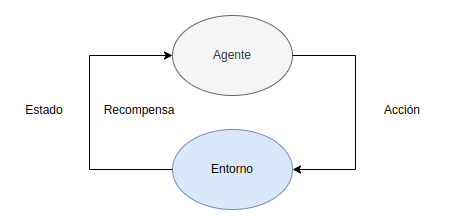
\includegraphics[width=0.9\textwidth]{diagrama.png}
	\captionof{figure}{Interacción entre el Agente y el entorno. }
	\label{fig:1}
\end{Figura}   

Antes del proceso de aprendizaje, $Q$ se inicializa a un posible valor arbitrario. Después, el Agente selecciona una acción en cada tiempo t, recibe una recompensa y llega a un nuevo estado, luego el valor de $Q$ se actualiza con base en la siguiente fórmula:
\begin{equation}
	\begin{split}
		\displaystyle	Q(s_t,a_t)  = &Q(s_t,a_t) + \\ & \alpha[r_{t+1} + \gamma \, max(Q(s_{t+1},a) - Q(s_t,a_t) )] \label{eq:1}
	\end{split}
\end{equation}
Donde $r_t$ representa la recompensa recibida cuando el Agente es transferido del estado $s_{t}$ al estado $s_{t+1}$. Y $\alpha$ representa la tasa de aprendizaje ($\alpha \in (0,1]$).

El objetivo del algoritmo aprendizaje por refuerzo (Q-learning) se actualiza siguiendo la fórmula:

\begin{equation}
	r_{t+1} + \gamma \, max Q(s_{t+1},a)
\end{equation} 

Y un episodio del algoritmo termina cuando el estado $s_{t+1}$ es terminal.

Los pasos específicos están detallados a continuación:

\begin{enumerate}[\hspace*{0.5cm} %
	\bfseries P{a}so 1]
	\item Inicializar $Q(s,a)$ arbitrariamente
	\item Establecer el parámetro $\gamma$ y $\alpha$
	\item Repetir (para cada episodio):
	\begin{enumerate}[1]
		\item Inicializar \textit{s}
		\item Repetir (para cada paso del episodio):
		\begin{enumerate}[2.1]
			\item Elegir \textit{a} desde \textit{s} usando una de las políticas de Q.
			\item Tomar la acción \textit{a}, observar r, $s'$
			\item $	\displaystyle	Q(s,a) \leftarrow Q(s,a) + \alpha[r + \gamma \, max(Q(s',a') - Q(s,a) )] $
			\item s $\leftarrow s'$ 
			\item Hasta que $s'$ sea terminal.
		\end{enumerate}
	\end{enumerate}
\end{enumerate}

La programación de taller de trabajo se divide en dos categorías funcionales \citep{zhao2019improved}:
\begin{enumerate}
	\item Selección de trabajo
	\item Selección de máquina.
\end{enumerate}
De acuerdo con los objetivos, las reglas de selección de trabajo y las reglas de selección de máquina se juntan; por lo tanto se necesita una regla de despacho de doble capa que incluya una capa para la selección de trabajo y una para la selección de máquina.

En la primer capa el conjunto de acciones son las siguientes \citep{zhao2019improved}:

\begin{enumerate}
	\item SPT: representa el mínimo de tiempo de procesamiento de las operaciones que serán seleccionados
	\item EDD: representa el mínimo de tiempo de entrega en las operaciones que serán seleccionadas
	\item FIFO: representa el primer trabajo en llegar que será seleccionado.
\end{enumerate}

La segunda capa se utiliza para seleccionar la máquina óptima de las máquinas alternativas según sus estados de procesamiento. Para simplificar el problema solo se seleccionará una regla de despacho definida como M, como la acción de la segunda capa que representa la máquina disponible más cercana que será seleccionada \citep{zhao2019improved}. 

La doble capa en grupo de acción incluye: SPT+M, EDD+M, FIFO+M, Ninguna.

Si se observa, el Agente realiza la selección en función de los estados; por lo tanto es muy importante determinar el número de estados, esto conlleva a dos resultados, por un lado si el número de estados es demasiado grande aumentarán en gran medida la carga calculada y por otro lado si es demasiada pequeña puede que no se adquiera el óptimo.

Una vez mencionado lo anterior se define SD como un indicador para establecer estados. SD es la relación de duración en que una máquina falla al tiempo total de procesamiento de las operaciones restantes en máquina fallida. La fórmula se describe a continuación:

\begin{equation}
	SD = \dfrac{100 \times T}{RT}
\end{equation}

Donde T es la duración en que la máquina falla y RT representa el tiempo total de procesamiento del resto de operaciones a partir de que la máquina falla. 

El Agente de aprendizaje por refuerzo (Q-learning) selecciona la mejor acción a juzgar de la recompensa (reward). Esto implica que la definición de recompensa es muy importante para el algoritmo. En el \fjsp \, el tiempo de espera representa uno de los factores más importantes a evaluar; por lo tanto se define la relación siguiente: ``entre más tiempo de espera menos es la recompensa" \citep{zhao2019improved}.

Los valores contemplados hasta el día de hoy si la acción seleccionada en SPT+M, EDD+M, FIFO+M y ninguna son: 2, 1, -1 y -2 respectivamente \citep{zhao2019improved}. 

La estructura del método propuesto se basa en la figura \ref{fig:2} \citep{zhao2019improved}.
\begin{Figura}
	\centering
	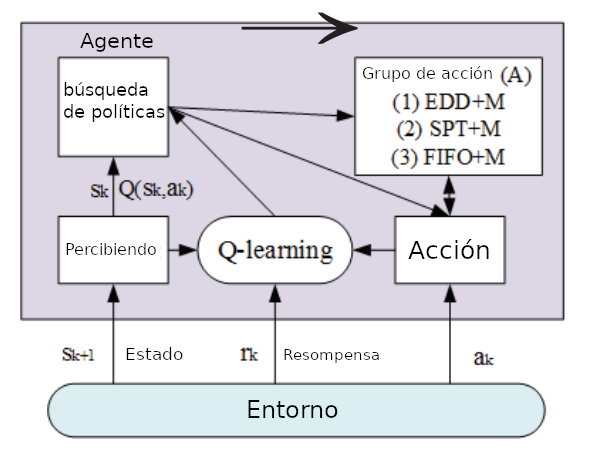
\includegraphics[width=0.9\textwidth]{estructura.png}
	\captionof{figure}{Estructura de la interacción del Agente dentro del entorno. }
	\label{fig:2}
\end{Figura}  
\section{Resultados}
\subsection{Esquema de planificación inicial basada en GA }
 Se inicia con una planificación basada en GA programada en python del problema Mk03 que es un caso típico de programación de taller de trabajo flexible presentado por \cite{brandimarte1993routing} citado por \cite{zhao2019improved}. El parámetro de la población es de 50, el número de iteraciones es de 500, y las probabilidades transversal y de mutación son 0.8 y 0.2 respectivamente.

A continuación se muestra el diagrama de Gantt del esquema de programación inicial
en la figura 3. Y se presenta la curva de variación de la función de aptitud en la figura 4 \citep{zhao2019improved}.

\begin{Figura}
	\centering
	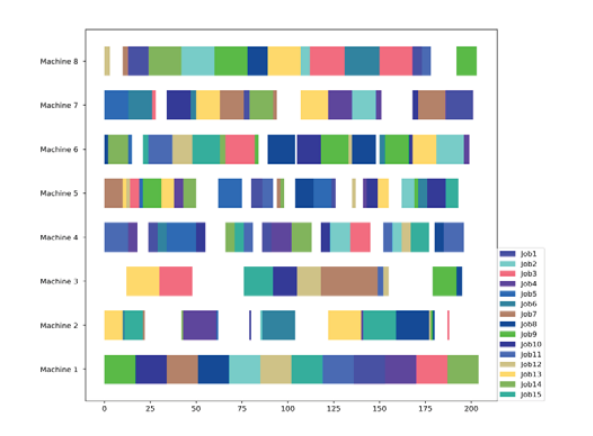
\includegraphics[width=0.9\textwidth]{GA-grafica.png}
	\captionof{figure}{Esquema inicial basado en GA.}
	\label{fig:3}
\end{Figura}  

\begin{Figura}
	\centering
	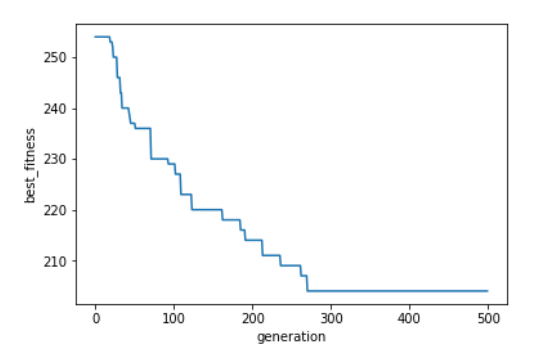
\includegraphics[width=0.9\textwidth]{fitness-generation.png}
	\captionof{figure}{La curva de variación de la función de aptitud.}
	\label{fig:4}
\end{Figura}  

\subsection{Planificación con base en aprendizaje por refuerzo (Q-learning)}

Se planea la obtención de distintos resultados variando cada una de las cuatro acciones que se tienen (SPT+M, EDD+M, FIFO+M y ninguna). Después de haber variado las acciones, se tiene contemplado el análisis simultáneo de las decisiones tomadas en cada acción. De acuerdo a los principios antes descritos de aprendizaje por refuerzo (Q-learning), si el agente obtiene una recompensa (reward) positiva el valor de $Q$ incrementa. Cuando el Agente selecciona su primer acción por ejemplo ninguna, el Agente archiva las recompensas positivas esto lo realiza de manera similar para las siguientes acciones. Teniendo los resultados en cada acción se evalúan los tiempos de las cuatro acciones, para concluir en un modelo de validación de nuestro algoritmo.

\section{Conclusiones}
Hasta el momento en que se escribe esta propuesta, la evidencia bibliográfica indica que el uso de un aprendizaje por refuerzo en un \fjsp \, tiene resultados muy favorables; sin embargo esta propuesta también planea explorar el tiempo computacional de dicho aprendizaje el cual ya se mencionó puede explotar en ciertas circunstancias.




\newpage
% \cite{CHEN2022939}

% \cite{Elvesier.com}
% \cite{Elvesier}
% \cite{european}
%\newpage
%\bibliographystyle{plain}
%\bibliography{bibliotarea1}
\bibliographystyle{apalike-es}
\bibliography{bibliotarea1}


\end{document}
%bibliografia 2: http://www2.psych.utoronto.ca/users/shkim/How%20to%20Write%20a%20Research%20Proposal.pdf
% bibliografia 3: https://www.ncbi.nlm.nih.gov/pmc/articles/PMC5037942/
%bibliografia https://www.ajol.info/index.php/njm/article/view/37249/25850
% biliografia 5:  https://www.researchgate.net/profile/Javed-Saani/publication/228983837_Learning_from_a_Doctoral_Research_Project_Structure_and_Content_of_a_Research_Proposal/links/53f55f8c0cf2888a7491bf23/Learning-from-a-Doctoral-Research-Project-Structure-and-Content-of-a-Research-Proposal.pdf
